
\section*{Problem 3}

\textit{Table.} From 2011 to 2020. All numbers are roud to four decimals.


\begin{table}[htbp]
    \centering
    \caption{The Annual Median for ROE and Total Revenue Growth Rate}
    \vspace{0.4cm}
    \csvautotabular{data/AS_1_p3_median.csv}
\end{table}

\ 


\textit{Graph.} From 2011 to 2020.

\begin{figure}[h]
\centering
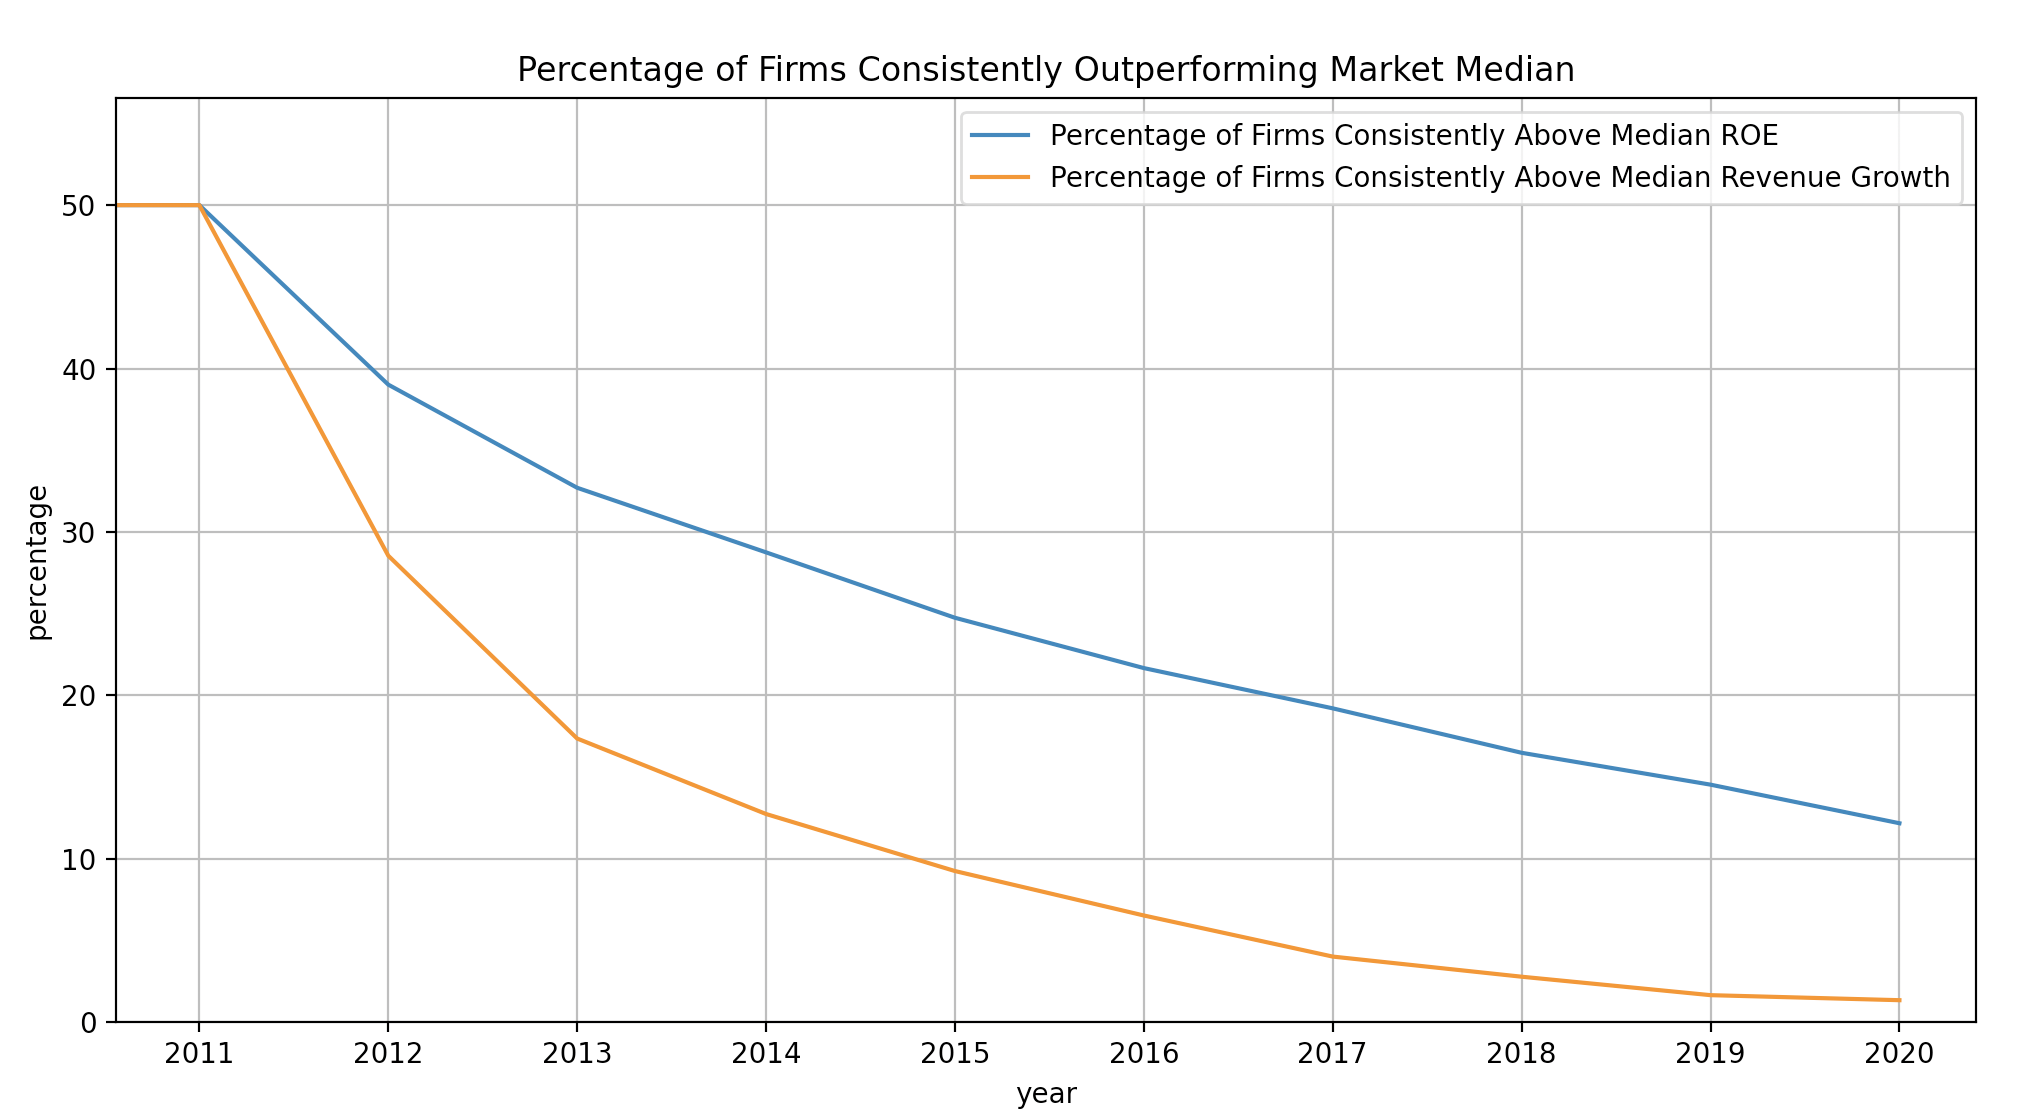
\includegraphics[width=1\textwidth]{data/pct_consistent_outperformer.png}
\caption{Time-series of the percentages of companies that consistently maintain above-median ROE and total revenue growth rate}
\label{fig:example}
\end{figure}

Noted that it represents the percentage of firms that outperform consistently than the median ROE and revenue growth rate, repectively.
